\documentclass{report}

\usepackage{inputenc}
\usepackage{fontenc}
\usepackage{array}
\usepackage{graphicx}
\usepackage[ngerman]{babel}
\usepackage{tabularx}
\usepackage{biblatex}
\usepackage{csquotes}
\usepackage{titling}
\usepackage{parskip}
\usepackage{placeins}
\usepackage{float}
\usepackage{geometry}
\usepackage{multirow}
\usepackage{rotating}
\usepackage{svg}
\usepackage{tabulary}
\usepackage{microtype}
\usepackage{titlesec}
\usepackage{svg}
\usepackage{makecell}
\usepackage{bytefield}

\usepackage{hyperref}

\addbibresource{.bib}

\geometry{a4paper, top=25mm, left=25mm, right=25mm, bottom=25mm}

\titleformat{\chapter}[display]
{\normalfont\huge\bfseries}
{}
{0pt}
{\Huge}

\setcounter{secnumdepth}{-1}

\title{\Huge{Gesammeltes Wissen} \\ \Large{in der Ausbildung zum Fachinformatiker Anwendungsentwicklung in Köln 2023 bis 2026}}
\author{Leon Ziegenhagen}
\date{Stand: \today}

\begin{document}

\maketitle

\tableofcontents

\chapter{Einleitung}

Dieses Dokument dient als Sammlung und Dokumentation des erlernten Wissens im Rahmen der Ausbildung zum Fachinformatiker in der Fachrichtung Anwendungsentwicklung. Es ist ein umfassender Überblick über die Ausbildungsinhalte, die im Verlauf der dreijährigen Berufsausbildung bei der AXA AG und insbesondere am Georg-Simon-Ohm Berufskolleg in Köln 2023 bis 2026 vermittelt wurden. Ziel dieses Dokumentes ist es, die wesentlichen Lerninhalte zu strukturieren und so eine verständliche Übersicht über die verschiedenen Fachthemen zu bieten, die während der Ausbildung behandelt wurden.

Dieses Dokument nennt hauptsächlich theoretisches Wissen, welches in der Berufsschule vermittelt wurde und oder welches von der IHK verlangt und geprüft wird.

\section{Duales System}

Für die Ausbildung ist das duale System vorgeschrieben. Diese hat sich in Deutschland ganz besonders erfolgreich erwiesen, da es den Auszubildenden ermöglicht, ihre theoretischen Kenntnisse in der Berufsschule mit praktischen Erfahrungen im Ausbildungsbetrieb zu kombinieren. Die Struktur des dualen Systems ist dabei klar gegliedert und findet auf verschiedenen Ebenen statt.

\begin{figure}[H]
    \centering
    \includesvg[width=1\textwidth,inkscapelatex=false]{figures/Duales_System.drawio.svg}
    \caption{Duales System}
    \label{fig:dualesSystem}
\end{figure}

% \includesvg[width=1\textwidth,inkscapelatex=false]{assets/uml_uc_01.svg}

Im Ausbildungsrahmenplan werden die Lernfelder wie in folgenden Kapiteln gegliedert. Darüber hinaus sieht das Land Nordrhein-Westfalen die Verknüpfung verschiedener Lernfelder in sog. Bündelungsfächer vor. Diese sind Gestaltung von IT-Dienstleistungen (GID), Wirtschaft- und Betriebslehre (WuB), Entwicklung vernetzter Prozesse (EvP), Cyber-Physische System (CPS), Softwaretechnologie und Datenmanagement (SuD) und IT-Grundrecht (ITG).

\begin{table}[H]
    \centering
    \begin{tabulary}{\textwidth}{|L|C|C|C|C|}
        \cline{2-5}
        \multicolumn{1}{c|}{} & GID \& WuB    & EvP \& CPS    & SuD   & ITG \\\hline
        LF 1            & X             &               &       &     \\\hline
        LF 2            & X             &               &       &     \\\hline
        LF 3            &               & X             &       &     \\\hline
        LF 4            &               &               &       & X   \\\hline
        LF 5            &               &               & X     &     \\\hline
        LF 6            & X             &               &       &     \\\hline
        LF 7            &               & X             &       &     \\\hline
        LF 8            &               &               & X     &     \\\hline
        LF 9            &               & X             &       &     \\\hline
        LF 10a          &               &               &       &     \\\hline
        LF 11a          &               &               &       &     \\\hline
        LF 12a          &               &               &       &     \\\hline
    \end{tabulary}
    \caption{Bündelungsfächer zu Lernfeldern}
    \label{tab:buendelfaecher}
\end{table}

\chapter{Lernfeld 1: Das Unternehmen und die eigene Rolle im Betrieb beschreiben}

\textbf{Die Schülerinnen und Schüler verfügen über die Kompetenz, ihr Unternehmen hinsichtlich seiner Wertschöpfungskette zu präsentieren und ihre eigene Rolle im Betrieb zu beschreiben.}

Die Schülerinnen und Schüler \textbf{informieren} sich, auch anhand des Unternehmensleitbildes,
über die ökonomischen, ökologischen und sozialen Zielsetzungen des Unternehmens.

Sie \textbf{analysieren} die Marktstruktur in ihrer Branche und ordnen das Unternehmen als komplexes System mit seinen Markt- und Kundenbeziehungen ein. Sie beschreiben die Wertschöpfungskette und ihre eigene Rolle im Betrieb.

Dabei erkunden sie die Leistungsschwerpunkte sowie Besonderheiten ihres Unternehmens
und setzen sich mit der Organisationsstruktur (Aufbauorganisation) und Rechtsform auseinander. Sie informieren sich über den eigenen Handlungs- und Entscheidungsspielraum im
Unternehmen (Vollmachten) sowie über Fort- und Weiterbildungsmaßnahmen.

Sie planen und \textbf{erstellen}, auch im Team, adressatengerecht multimediale Darstellungen zu
ihrem Unternehmen.

Die Schülerinnen und Schüler \textbf{präsentieren} ihre Ergebnisse.

Sie \textbf{überprüfen} kriteriengeleitet die Qualität ihres Handlungsproduktes und entwickeln gemeinsam Verbesserungsmöglichkeiten.

Sie \textbf{reflektieren} die eigene Rolle und das eigene Handeln im Betrieb.

\section{Unternehmensleitbild}

Ein Unternehmensleitbild beschreibt das Selbstverständnis und die Grundsätze eines Unternehmens. Es richtet sich an Mitarbeiter, Kunden und an die Öffentlichkeit. Es beinhaltet:

\begin{itemize}
    \item Vision / Selbstverständnis
    \item Mission / Ziel
    \item Grundsätze / Strategie
\end{itemize}

Das Leitbild verdeutlicht den Sinn und Zweck des Unternehmens und trägt zur Imagepflege bei. Ein erfolgreiches Leitbild sollte folgendes bewirken:

\begin{itemize}
    \item Motivierte und unternehmen-gebundene Mitarbeiter
    \item Grundlage für Unternehmensziele und Strategien
    \item Klare und zur Konkurrenz differenzierte Unternehmensidentität
    \item Entscheidungshilfe für Führungskräfte
    \item Hilfestellung in Konfliktsituationen
    \item Vereinfachte Personalauswahl
\end{itemize}

\section{Unternehmensziele}

Unternehmensziele leiten sich oft aus den im Unternehmensleitbild formulierten Grundsätzen und Visionen ab. Unternehmensziele sollten allerdings konkret und messbar ausformuliert werden. Diese Ziele lassen sich folgendermaßen kategorisieren:

\begin{itemize}
    \item Sachziele
    \item Ökonomische Ziele
    \item Ökologische Ziele
    \item Soziale Ziele
\end{itemize}

Dabei sind erwerbswirtschaftliche Unternehmen i.d.R. an Gewinnmaximierung, Rentabilität und oder hohem Marktanteil interessiert wohingegen öffentliche Unternehmen i.d.R. an Bedarfsdeckung, Kostendeckung, Verlustminimierung und oder angemessenem Gewinn interessiert sind. Der Aspekt Nachhaltigkeit ist für alle Unternehmen unter den Aspekten des Images, des Umsatzes, der Kostensenkung und der ökologisch-sozialen Verantwortung interessant.

Unternehmensziele können komplementär, konkurrierend oder neutral einander gegenüberstehen.

\section{Shareholder und Stakeholder}

Shareholder sind Anteilseigner bzw. Kapitalgeber. Stakeholder sind unabhängig von ihrer finanzielle Beteiligung Einflussnehmer oder Betroffene von (Teil-)Unternehmen.

\section{Aufbauorganisation}
Die Aufbauorganisation bestimmt welche Aufgaben von welchen Personen übernommen werden. Sie grenzt sich von der Ablauforganisation ab, welche den Ablauf von Leistungs- und Produktionsprozessen bestimmt. Um eine Aufbauorganisation darzustellen bieten sich Leitungssysteme an, welche speziell Führungs- und Entscheidungsprozesse im Unternehmen organisieren. Die grafische Darstellung eines Leitungssystem ist z.B. das sog. Organigramm, welches zusätzlich Abteilungen oder Teams darstellen kann.

Leistungssysteme lassen sich folgendermaßen differenzieren:

\begin{table}[H]
    \centering
    \begin{tabularx}{\textwidth}{|>{\raggedright\arraybackslash}l|>{\raggedright\arraybackslash}X|>{\raggedright\arraybackslash}X|>{\raggedright\arraybackslash}X|>{\raggedright\arraybackslash}X|}
        \hline
                   & Einliniensystem                                                                                                                                          & Stab-Liniensystem                                                                                                                 & Mehrliniensystem (Funktional)                                                                                                                                                                                                                             & Matrixsystem                                                                                                                                                                                                                                                        \\
        \hline
        Grundsatz  & Eine untergeordnete Stelle erhält jeweils nur von einer vorgesetzten Instanz Anweisungen. Die Linie bildet gleichzeitig den kommunikativen Dienstweg ab. & Ein um Stäbe erweitertes Einliniensystem. Die Stäbe haben keine Weisungsbefugnis sondern bereiten Entscheidungen vor und beraten. & Spezialisten sind für definierte Funktionen zuständig und unmittelbar fachlich weisungsbefugt. Anforderungen bzw. Anweisungen können von verschiedenen Vorgesetzten kommen und Instanzen auf gleicher Ebene können unmittelbar miteinander kommunizieren. & Es existieren zwei weitestgehend unabhängige Hierarchien o. Dimensionen. Z.B. können Funktionen und Objekte oder Projekte sein. An Kreuzungspunkten befinden sich fachliche Spezialisten, welche Anforderungen von überall bekommen können, aber meist autark sind. \\
        \hline
        Schema     & siehe Abb. \ref{fig:einliniensystem}                                                                                                                     & siehe Abb. \ref{fig:stabliniensystem}                                                                                             & siehe Abb. \ref{fig:mehrliniensystem}                                                                                                                                                                                                                     & siehe Abb. \ref{fig:matrixsystem}                                                                                                                                                                                                                                   \\
        \hline
        Eigenarten & Streng hierarchisches Denken und große Macht bei Leitungskräften.                                                                                        & Trennung von Entscheidungs- und Fachkompetenz.                                                                                    & Spezialisierung der Instanzen und verkürzte Delegations- und Informationswege.                                                                                                                                                                            & Autarke und schnell agierende Instanzen.                                                                                                                                                                                                                            \\
        \hline
        Vorteile   & klare Zuständigkeiten, einfach, Konflikte wg. widersprüchlichen Anweisungen unwahrscheinlich                                                             & Entlastung der Führungskräfte, Trennung und Konzentration Entscheidungs- und Fachkompetenzen                                      & höhere Flexibilität, schnellere Entscheidungsfindung, Entlastung durch Spezialisierung der Führungskräfte                                                                                                                                                 & optimierte Ressourcennutzung, Flexibilität und Dynamik, Förderung interdisziplinärer Zusammenarbeit                                                                                                                                                                 \\
        \hline
        Nachteile  & hohe Last bei Führungskräften, geringe Flexibilität, lange Kommunikationswege                                                                            & mögliche unklare Verantwortungen, Konfliktmöglichkeit zwischen Führungskraft und Stab                                             & hohes Konfliktpotential zwischen Führungskräften, unklare Verantwortlichkeiten, Komplexität                                                                                                                                                               & Konfliktpotential zwischen Führungskräften, Komplexität insbesondere der Kommunikation und Koordination, Hoher Abstimmungsaufwand für die Gesamtunternehmensplanung                                                                                                 \\
        \hline
    \end{tabularx}
    \caption{Leitungssysteme}
    \label{tab:leitungssysteme}
\end{table}


\begin{figure}[H]
    \centering
    \includesvg[width=\textwidth,inkscapelatex=false]{figures/Einliniensystem.drawio.svg}
    \caption{Einliniensystem}
    \label{fig:einliniensystem}
\end{figure}
\FloatBarrier

\begin{figure}[H]
    \centering
    \includesvg[width=\textwidth,inkscapelatex=false]{figures/Stabliniensystem.drawio.svg}
    \caption{Stab-Liniensystem}
    \label{fig:stabliniensystem}
\end{figure}
\FloatBarrier

\begin{figure}[H]
    \centering
    \includesvg[width=\textwidth,inkscapelatex=false]{figures/Mehrliniensystem.drawio.svg}
    \caption{Mehrliniensystem}
    \label{fig:mehrliniensystem}
\end{figure}
\FloatBarrier

\begin{figure}[H]
    \centering
    \includesvg[width=\textwidth,inkscapelatex=false]{figures/Matrixsystem.drawio.svg}
    \caption{Matrixsystem}
    \label{fig:matrixsystem}
\end{figure}
\FloatBarrier

\section{Rechtsformen}

Rechtsformen beziehen sich auf Unternehmen. Unternehmen sind dabei von Betrieben und Firmen folgendermaßen abzugrenzen. Unternehmen sind rechtlich selbstständige organisatorische Einheiten der Volkswirtschaft. Betriebe sind technisch-soziale Einheiten und Unternehmen unterzuordnen. Betriebe beschreiben oft örtliche Einheiten eines Unternehmens. Firmen sind im Handelsregister eingetragene Namen eines Unternehmens. Sie bestehen aus Firmenkern (eigentlicher Name) und Firmenzusatz (Rechtsform).

Der Firmenkern kann sich von Namen (Personenfirmenkern), von Produkten oder Dienstleistungen (Sachfirmenkern), aus einer Mischform (Mischfirmenkern) ableiten oder frei erfunden werden (Fantasie-Firmenkern).

\textbf{Einzelunternehmen}

Der einzelne Unternehmer (eigentragener Kaufmann (E.K.)) hat alleiniges Bestimmungsrecht. Er bringt das gesamte notwendige Kapital auf und erhält den kompletten Gewinn. Er trägt das alleinige Risiko und haftet mit seinem gesamten Betriebs- und Privatvermögen. Es ist die häufigste Rechtsform in Deutschland.

\textbf{Personengesellschaften}

Personengesellschaften werden von mindesten zwei i.d.R. natürlichen Personen gegründet. Zu Personengesellschaften gehören u.a. die Gesellschaft bürgerlichen Rechts (GbR), die offene Handelsgesellschaft (OHG) und die Kommanditgesellschaft (KG). Gesellschafter haften für Gesellschaftsschulden persönlich. Gesellschafter sind Inhaber und meist auch Geschäftsführer.

\textbf{Kapitalgesellschaften}

Kapitalgesellschaften sind z.B. die Gesellschaft mit beschränkter Haftung (GmbH) und die Aktiengesellschaft (AG). Die Haftung ist auf Gesellschaftseinlagen beschränkt. Für die Gründung ist ein Mindestkapital notwendig. Kapitalgesellschaften sind juristische Personen und können von beliebigen Personen geführt werden.

\begin{table}[H]
    \centering
    \begin{tabularx}{\textwidth}{|>{\raggedright\arraybackslash}l|>{\raggedright\arraybackslash}X|>{\raggedright\arraybackslash}X|>{\raggedright\arraybackslash}l|>{\raggedright\arraybackslash}X|>{\raggedright\arraybackslash}X|}
        \hline
             & Mindest\-Gründerzahl              & Haftung                                                                                                        & Mindest\-kapital & Geschäfts\-führung                                                        & Gewinn\-verteilung                                                                                                                                      \\
        \hline
        E.K. & 1                                 & unbeschränkt inkl. Privatvermögen                                                                              & -                & Eingetragener Kaufmann                                                    & Voller Gewinn an den Eingetragenen Kaufmann                                                                                                             \\
        \hline
        GbR  & 2                                 & unbeschränkt inkl. Privatvermögen                                                                              & -                & alle Gesellschafter, sofern im Gesellschaftsvertrag nicht anders geregelt & zu gleichen Teilen auf alle Gesellschafter, sofern im Gesellschaftsvertrag nicht anders geregelt                                                        \\
        \hline
        OHG  & 2                                 & unbeschränkt inkl. Privatvermögen                                                                              & -                & alle Gesellschafter, sofern im Gesellschaftsvertrag nicht anders geregelt & min. 4\% der Einlagen eines Gesellschafters und danach zu gleichen Teilen auf alle Gesellschafter, sofern im Gesellschaftsvertrag nicht anders geregelt \\
        \hline
        KG   & 1 Komplementär und 1 Kommanditist & Betriebs\-vermögen, dann Einlagen der Kommanditisten und zuletzt der Komplementär inkl. seines Privatvermögens & -                & Alle Komplementäre                                                        & min. 4\% der Einlagen eines Gesellschafters und danach oder anstelle davon durch vertragliche Regelungen                                                \\
        \hline
        GmbH & 1                                 & beschränkt auf das Gesellschaftsvermögen                                                                       & 25.000€          & Angestellter Geschäftsführer                                              & Gewinnanteil entsprechend des Kapitalanteils, sofern vertraglich nicht anders geregelt                                                                  \\
        \hline
        AG   & 1                                 & beschränkt auf das Gesellschaftsvermögen                                                                       & 50.000€          & Vorstand                                                                  & Gewinnanteil entsprechend des Aktienanteil oder vertraglich geregelt z.B. mit Dividenden                                                                \\
        \hline
    \end{tabularx}
    \caption{Rechtsformen}
    \label{tab:rechtsformen}
\end{table}

Es gibt außerdem Mischformen wie die GmbH \& Co. KG, bei welcher eine KG von u.a. einer GmbH gegründet wird.

\section{Handelsregister}

Das Handelsregister verzeichnet Kaufleute und Firmen. Abteilung A registriert Einzelunternehmen und Personengesellschaften. Abteilung B registriert Kapitalgesellschaften.

\section{Vollmachten und Prokura}

Prokura ist eine Vertretungsmacht zur Geschäftsführung deren Umfang gesetzlich geregelt ist. Handlungsvollmachten begrenzen sich dagegen auf bestimmte Geschäfte.

Handlungsvollmacht ist dabei ein Oberbegriff für Generalhandlungsvollmachten und allgemeine Vollmachten, welche zum Führen des täglichen Geschäftes ermächtigen, Artvollmachten, welche sich auf einen finanziellen Rahmen oder auf einen bestimmten Handlungsbereich beschränken und Sondervollmachten, welche einmalig für explizite Geschäfte erteilt werden.

\section{Eigene Rolle im Betrieb}

Die eigene Rolle im Betrieb ist vorwiegend durch Rechte und Pflichten in der Ausbildung geprägt. Vor allem herrschen hier die Grundsätze des Individualrechts:

\subsection{Berufsbildungsgesetz (BBiG)}

Die Berufsbildung wird in Betrieben und in Berufsschulen kooperativ durchgeführt (§2 Abs. 1 und 2 BBiG).

Die Form und geforderte Inhalte einer Ausbildungsordnung ist definiert (§5 BBiG). Die Ausbildungsordnung für Fachinformatiker ist weiter unten unter FIAusbV beschrieben.

Es muss ein Ausbildungsvertrag geschlossen werden (§10 BBiG). Dieser muss folgendes beinhalten (§11 BBiG):

\begin{itemize}
    \item Name und Anschrift der Vertragsparteien
    \item Art, sachliche und zeitliche Gliederung und Ziel der Ausbildung
    \item Beginn und Dauer
    \item Ausbildungsstätte und Ausbildungsnahmen außerhalb
    \item tägliche Arbeitszeit
    \item Probezeit
    \item Vergütung
    \item Umgang mit Überstunden
    \item Urlaub
    \item Voraussetzungen für Kündigung
    \item Form des Ausbildungsnachweises
\end{itemize}

Folgende Vereinbarung sind in einer Ausbildung nichtig (§12 BBiG):

\begin{itemize}
    \item Verpflichtung zur Übernahme (außer 6 Monate vor Ausbildungsende)
    \item Verpflichtung zur Entschädigungszahlung für die Ausbildung
    \item Vertragsstrafen
    \item Ausschluss oder Beschränkung von Schadensersatzansprüchen inkl. der Festsetzung von Pauschalen bei Schadensersatz
\end{itemize}

Pflichten des Auszubildenden sind u.a. (§13 BBiG):

\begin{itemize}
    \item sorgfältig Aufgaben auszuführen
    \item Ausbildungsmaßnahmen wahrzunehmen, für welche Sie freigestellt werden
    \item Weisungen befolgen
    \item Ausbildungsstättenordnung beachten
    \item Werkzeug, Maschinen und sonstiges pfleglich behandeln
    \item Schweigepflicht über Betriebsgeheimnisse
    \item schriftlichen oder elektronischen Ausbildungsnachweis führen
\end{itemize}

Pflichten des Ausbildenden sind u.a. (§14 BBiG):

\begin{itemize}
    \item nach bestem Gewissen für den Beruf auszubilden
    \item selbst auszubilden oder ausdrücklich einen Ausbilder beauftragen
    \item Ausbildungsmittel kostenlos zur Verfügung stellen
    \item Auszubildende zum Besuch der Berufsschule anzuhalten
    \item Charakter des Auszubildenden fördern und körperliche Gefahren vermeiden
    \item Auszubildende zum Führen des Ausbildungsnachweises anzuhalten und diesen regelmäßig durchzusehen
    \item nur Aufgaben stellen, welche dem Ausbildungszweck dienen und den körperlichen Kräften des Auszubildenden angemessen sind
\end{itemize}

Auszubildende sind für die Berufsschule und Prüfungen freizustellen (§15 Abs. 1 und 2 BBiG). Für volljährige Auszubildende gilt:

\begin{table}[H]
    \centering
    \begin{tabularx}{\textwidth}{|>{\raggedright\arraybackslash}X|>{\raggedright\arraybackslash}X|}
        \hline
        Situation und Freistellung                                                                   & Anrechnung der Arbeitszeit                                                                           \\
        \hline
        Berufsschulunterricht                                                                        & Unterrichts- und Pausenzeit und notwendige Wegzeiten zwischen Berufsschule und Ausbildungsstätte     \\
        \hline
        ein Berufsschultag in der Woche mit mehr als 5 Unterrichtsstunden á 45 Min                   & durchschnittliche tägliche Arbeitszeit                                                               \\
        \hline
        Berufsschulwochen mit einem planmäßigen Blockunterricht von mindestens 25 Stunden an 5 Tagen & durchschnittliche wöchentliche Arbeitszeit                                                           \\
        \hline
        Prüfungen und Ausbildungsmaßnahmen                                                           & Zeit der Teilnahme inkl. Pausen und notwendige Wegzeiten zwischen Teilnahmeort und Ausbildungsstätte \\
        \hline
        Arbeitstag vor der AP 2                                                                      & durchschnittliche tägliche Arbeitszeit                                                               \\
        \hline
    \end{tabularx}
    \caption{Freistellung, Anrechnung}
    \label{tab:freistellung}
\end{table}

Der Ausbildende hat bei Beendigung ein Arbeitszeugnis auszustellen (§16 BBiG).

Auszubildende haben ein Anrecht auf eine Mindestvergütung mit jedem Lehrjahr steigend (§17 BBiG).

Die Probezeit darf zwischen einem und vier Monaten dauern (§20 BBiG).

Die Ausbildung endet mit Ablauf der Ausbildungsdauer oder bei bestehen der Abschlussprüfung mit Bekanntgabe der Ergebnisse (§21 Abs. 1 und 2 BBiG). Der Auszubildende kann bei nicht bestehen Verlangen das Ausbildungsverhältnis bis zur nächstmöglichen Prüfungswiederholung zu verlängern, maximal aber ein Jahr (§21 Abs. 3 BBiG).

Während der Probezeit kann jederzeit und ohne Frist gekündigt werden (§22 Abs. 1 BBiG). Nach der Probezeit darf nur aus einem wichtigen Grund und ohne Frist gekündigt werden oder vom Auszubildenden mit einer Frist von vier Wochen, wenn Sie die Ausbildung aufgeben oder eine andere Berufstätigkeit ausüben wollen (§22 Abs. 2 BBiG). Kündigungen müssen schriftlich sein und außerhalb der Probezeit den Kündigungsgrund beinhalten (§22 Abs. 3 BBiG). Eine Kündigung aus wichtigem Grund ist unwirksam, wenn dieser dem Kündigungsberechtigten länger als zwei Woche bekannt ist, außer es ist ein Güteverfahren eingeleitet, welches die Frist hemmt (22 Abs. 4 BBiG).

Werden Auszubildende nach Abschluss der Ausbildung beschäftigt ohne ausdrückliche Vereinbarung, so liegt automatisch ein Arbeitsverhältnis auf unbestimmte Zeit vor (§24 BBiG).

Die Abschlussprüfung kann bis zu zweimal wiederholt werden und ist für Auszubildende gebührenfrei. Es muss ein Zeugnis ausgestellt werden (§37 BBiG).

\subsection{Fachinformatikerausbildungsverordnung (FIAusbV)}

Die Ausbildung dauert 3 Jahre (§2 FIAusbV).

Gliederung in die Fachrichtungen Anwendungsentwicklung, Systemintegration, Daten- und Prozessanalyse und Digitale Vernetzung (§4 Abs. 1 Satz 2 FIAusbV).

Regelungen zur Abschlussprüfung finden sich in den §§ 7 bis 41 FIAusbV.

\subsection{Bundesurlaubsgesetz (BUrlG)}

U.a. als volljähriger Auszubildender hat man einen Anspruch auf bezahlten Urlaub von mindestens 24 Werktagen pro vollem Jahr (§§ 1 bis 3 BUrlG).

\subsection{Arbeitsschutzgesetz (ArbSchG)}

Der Arbeitgeber hat Gefahren für den Arbeitnehmer bestmöglich zu vermeiden oder gering zu halten, in dem er Maßnahmen des Arbeitsschutzes trifft und generell eine Verbesserung von Sicherheit und Gesundheitsschutz anstrebt. Der Arbeitgeber hat den Arbeitnehmer zu unterweisen und der Arbeitnehmer hat sich möglichst an die Unterweisungen und Weisungen für seinen Schutz zu halten.

\subsection{Arbeitszeitgesetz (ArbZG)}

Die werktägliche Arbeitszeit ist max. acht Stunden. Sie kann auf zehn Stunden verlängert werden, wenn die durchschnittliche Arbeitszeit innerhalb von 24 Wochen acht Stunden werktäglich nicht überschreitet (§3 ArbZG).

Ab einer Arbeitszeit von sechs Stunden bis zu neun Stunden sind voraus feststehende Ruhepausen von insgesamt mindestens 30 Min. und ab einer Arbeitszeit ab neun Stunden Ruhepausen von insgesamt mindestens 45 Min. einzulegen. Eine Ruhepause muss min. 15 Minuten betragen. Es darf nicht länger als sechs Stunden ohne Ruhepause gearbeitet werden (§4 ArbZG).

Zwischen den Arbeitszeiten muss eine Ruhezeit von mindestens elf Stunden liegen (§5 Abs. 1 ArbZG).

Es gilt ein generelles Beschäftigungsverbot an Sonn- und Feiertagen (§9 Abs. 1 ArbZG).

Es existieren definierte Ausnahmen und abweichende Regelungen.

\subsection{Mutterschutzgesetz (MuSchG)}

Eine schwangere Frau darf in den letzten sechs Wochen vor der Entbindung nur mit ihrem ausdrücklichen Wunsch beschäftigt werden (§3 Abs. 1 MuSchG).

Nach der Entbindung darf eine Frau acht Wochen nicht beschäftigt werden (§3 Abs. 2 MuSchG), außer auf ausdrücklichen Wunsch in schulischen oder hochschulischen Ausbildungen (§3 Abs. 3 MuSchG).

Einer schwangeren oder stillenden Frau ist Mehrarbeit verboten (§4 MuSchG), sowie generell die Nachtarbeit (§5 MuSchG) und generell die Arbeit an Sonn- und Feiertagen (§6 MuSchG).

Eine schwangere Frau oder Mutter ist für entsprechende Untersuchungen freizustellen(§7 Abs. 1 MuSchG).

Eine stillende Frau hat Anspruch auf Freistellung zum Stillen in den ersten zwölf Monaten nach der Entbindung (§7 Abs 2. MuSchG).

Während der Schwangerschaft und min. vier Monate nach der Entbindung darf eine Frau nicht gekündigt werden (§17 MuSchG).

\subsection{Jugendarbeitsschutzgesetz (JArbSchG)}

\subsection{Bundeselterngeld- und Elternzeitgesetz (BEEG)}

\subsection{Sozialgesetzbuch 9 (SGB IX)}

\subsection{Allgemeines Gleichbehandlungsgesetz (AGG)}

\subsection{Sonstige}

Es sind u.a. auch das Kündigungsschutzgesetz (KSchG) und die Arbeitsstättenverordnung (ArbStättV) zu beachten.

\chapter{Lernfeld 2: Arbeitsplätze nach Kundenwunsch ausstatten}

\textbf{Die Schülerinnen und Schüler verfügen über die Kompetenz, die Ausstattung eines
    Arbeitsplatzes nach Kundenwunsch zu dimensionieren, anzubieten, zu beschaffen
    und den Arbeitsplatz an die Kunden zu übergeben.}

Die Schülerinnen und Schüler nehmen den Kundenwunsch für die Ausstattung eines Arbeitsplatzes von internen und externen Kunden entgegen und \textbf{ermitteln} die sich daraus
ergebenden Anforderungen an Soft- und Hardware. Aus den dokumentierten Anforderungen leiten sie Auswahlkriterien für die Beschaffung ab. Sie berücksichtigen dabei die Einhaltung von Normen und Vorschriften (Zertifikate, Kennzeichnung) für den Betrieb und die
Sicherheit von elektrischen Geräten und Komponenten.

Sie \textbf{vergleichen} die technischen Merkmale relevanter Produkte anhand von Datenblättern
und Produktbeschreibungen zur Vorbereitung einer Auswahlentscheidung (Nutzwertanalyse). Dabei beachten sie insbesondere informationstechnische und energietechnische
Kenngrößen sowie Aspekte der Ergonomie und der Nachhaltigkeit (Umweltschutz, Recycling). Sie wenden Recherchemethoden an und werten auch fremdsprachliche Quellen aus.

Sie ermitteln die Energieeffizienz unterschiedlicher Arbeitsplatzvarianten und dokumentieren diese.

Sie vergleichen mögliche Bezugsquellen (quantitativer und qualitativer Angebotsvergleich)
und \textbf{bestimmen} den Lieferanten.

Auf Basis der ausgewählten Produkte und Lieferanten \textbf{erstellen} sie mit vorgegebenen Zuschlagssätzen ein Angebot für die Kunden.

Sie schließen den Kaufvertrag ab und organisieren den Beschaffungsprozess unter Berücksichtigung von Lieferzeiten. Sie nehmen die bestellten Komponenten in Empfang und dokumentieren dabei festgestellte Mängel.

Sie bereiten die Übergabe der beschafften Produkte vor, integrieren IT-Komponenten, konfigurieren diese und nehmen sie unter Berücksichtigung der Arbeitssicherheit in Betrieb. Sie
übergeben den Arbeitsplatz an die Kunden und erstellen ein Übergabeprotokoll.

Sie \textbf{bewerten} die Durchführung des Kundenauftrags und \textbf{reflektieren} ihr Vorgehen. Dabei
berücksichtigen sie die Kundenzufriedenheit und formulieren Verbesserungsvorschläge.

\section{Nutzwertanalyse}
Die Nutzwertanalyse (NWA) ist eine Methode des qualitativen (Angebots-)Vergleich, indem unterschiedlich bestimmte Teilnutzen zu einem Gesamtnutzen addiert werden, welcher gegen Alternativen verglichen werden kann.

\textbf{Vorgehensweise}

\begin{enumerate}
    \item Festlegen der Bewertungskriterien / Teilnutzenaspekten
    \item Festlegen der Gewichtungsfaktoren / Anteile der einzelnen Bewertungskriterien
    \item Aufstellen einer Punkteskala (z.B. Schulnoten, 0-10, 0-100)
    \item Bewertung der Entscheidungsalternativen anhand der Skala
    \item Ermitteln der gewichteten Punktwerte als Produkt aus Bewertung und Gewichtungsfaktor
    \item Summieren der gewichteten Punktwerte
    \item Interpretation der Ergebnisse
\end{enumerate}

\textbf{Beispiel}

\begin{table}[H]
    \centering
    \begin{tabularx}{\textwidth}{|>{\arraybackslash}X|c|>{\centering\arraybackslash}X|>{\centering\arraybackslash}X|>{\centering\arraybackslash}X|>{\centering\arraybackslash}X|>{\centering\arraybackslash}X|>{\centering\arraybackslash}X|}
        \hline
                    &       & \multicolumn{2}{c|}{Unternehmen 1} & \multicolumn{2}{c|}{Unternehmen 2} & \multicolumn{2}{c|}{Unternehmen 3}                                      \\
        \hline
                    & Gew.  & Punkte                             & Gew. Punkte                        & Punkte                             & Gew. Punkte & Punkte & Gew. Punkte \\
        \hline
        Grafikkarte & 20\%  & 3                                  & 60                                 & 2                                  & 40          & 4      & 80          \\
        \hline
        RAM         & 25\%  & 4                                  & 100                                & 3                                  & 75          & 4      & 100         \\
        \hline
        Monitor     & 40\%  & 2                                  & 80                                 & 1                                  & 40          & 4      & 160         \\
        \hline
        Preis       & 15\%  & 3                                  & 45                                 & 4                                  & 60          & 1      & 15          \\
        \hline
                    & 100\% &                                    & 285                                &                                    & 215         &        & 355         \\
        \hline
    \end{tabularx}
    \caption{Beispiel Nutzwertanalyse}
    \label{tab:nutzwertanalyse}
\end{table}

Die Bewertungskriterien bilden das jeweilige Teilnutzen ab. Die Größe eines Nutzens bemisst sich an denjenigen, welche das Gut nutzen, den Zweck, die Situation, der Zeitpunkt und das Gut selbst. Die Bewertungskriterien sollte untereinander nutzenunabhängig sein.

\textbf{Vorteile}

\begin{itemize}
    \item Flexibilität
    \item Schnelligkeit
    \item direkter Vergleich
    \item Eindeutigkeit
\end{itemize}

\textbf{Nachteile}

\begin{itemize}
    \item Subjektivität
    \item Manipulierbarkeit
    \item Ausschluss von Konsequenzen
    \item Niedrige Aussagekraft bei Alternativen mit sehr ähnlichen quantitativen Gesamtnutzen
\end{itemize}

\section{Handelskalkulation}

Die Handelskalkulation wird intern in Netto berechnet. Der Listeneinkaufspreis und Listenverkaufspreis muss für außen also ggf. in Brutto umgerechnet werden.

\subsection{Bezugskalkulation}

\begin{table}[H]
    \centering
    \begin{tabular}{c|l}
          & Listeneinkaufspreis (LEP)       \\
        \hline
        - & Lieferrabatt                    \\
        \hline
        = & Zieleinkaufspreis (ZEP)         \\
        \hline
        - & Lieferskonto                    \\
        \hline
        = & Bareinkaufspreis (BEP)          \\
        \hline
        + & Bezugskosten (z.B Lieferkosten) \\
        \hline
        = & Bezugspreis / Einstandspreis    \\
    \end{tabular}
    \caption{Bezugskalkulation}
\end{table}

\subsection{Quantitativer Angebotsvergleich}

Mithilfe der Bezugskalkulation wird häufig ein quantitativer Angebotsvergleich durchgeführt. Dabei wird der Bezugspreis der verschiedenen Anbieter verglichen, um den günstigsten Anbieter zu ermitteln.

\subsection{Selbstkostenkalkulation im Handel}

\begin{table}[H]
    \centering
    \begin{tabular}{c|l}
          & Bezugspreis     \\
        \hline
        + & Handlungskosten \\
        \hline
        = & Selbstkosten    \\
    \end{tabular}
    \caption{Selbstkostenkalkulation}
\end{table}

Handlungskosten sind alle Kosten im Unternehmen, welche nicht direkt dem Bezug von Ware zugeordnet werden können (z.B Personalkosten, Miete, Steuer). Handlungskosten werden meist prozentual als Handlungskostenzuschlag auf den Bezugspreis aufgeschlagen. Der Handlungskostenzuschlag ist dabei das Verhältnis von Handlungskosten zu Warenaufwänden in einer Periode.

\subsection{Verkaufskalkulation}

\begin{table}
    [H]
    \centering
    \begin{tabular}{c|l}
          & Selbstkosten              \\
        \hline
        + & Gewinn                    \\
        \hline
        = & Barverkaufspreis (BVP)    \\
        \hline
        + & Kundenskonto              \\
        \hline
        = & Zielverkaufspreis (ZVP)   \\
        \hline
        + & Kundenrabatt              \\
        \hline
        = & Listenverkaufspreis (LVP) \\
    \end{tabular}
    \caption{Verkaufskalkulation}
\end{table}

Achtung! Der Kundenskonto bezieht sich auf den Zielverkaufspreis und nicht den Barverkaufspreis. Der Kundenrabatt bezieht sich auf den Listenverkaufspreis und nicht den Zielverkaufspreis.

Es gilt:

\begin{center}
    $ZVP = BVP + \frac{BVP * Kundenskonto}{100\% - Kundenskonto}$
\end{center}

und

\begin{center}
    $LVP = ZVP + \frac{ZVP * Kundenrabatt}{100\% - Kundenrabatt}$
\end{center}

\subsection{Vollständige Handelskalkulation Vorwärts}

Die Vorwärtskalkulation eignet sich für Märkte mit freier Preisgestaltung.

\begin{table}
    [H]
    \centering
    \begin{tabular}{c|l}
          & Listeneinkaufspreis (LEP) \\
        \hline
        - & Lieferrabatt              \\
        \hline
        = & Zieleinkaufspreis (ZEP)   \\
        \hline
        - & Lieferskonto              \\
        \hline
        = & Bareinkaufspreis (BEP)    \\
        \hline
        + & Bezugskosten              \\
        \hline
        = & Bezugspreis               \\
        \hline
        + & Handlungskosten           \\
        \hline
        = & Selbstkosten              \\
        \hline
        + & Gewinn                    \\
        \hline
        = & Barverkaufspreis (BVP)    \\
        \hline
        + & Kundenskonto              \\
        \hline
        = & Zielverkaufspreis (ZVP)   \\
        \hline
        + & Kundenrabatt              \\
        \hline
        = & Listenverkaufspreis (LVP) \\
    \end{tabular}
    \caption{Vollständige Handelskalkulation Vorwärts}
\end{table}

Siehe Verkaufskalkulation für die Berechnung von ZVP und LVP.

\subsection{Rückwärtskalkulation}

Die Rückwärtskalkulation eignet sich für Märkte mit vorgegebenen Verkaufspreisen.

Das Schema der Rückwärtskalkulation ist gleich dem Schema der Vorwärtskalkulation. Allerdings ist letztere Umzudrehen, Vorzeichen werden invertiert und die besondere Berechnung vo ZVP und LVP wie in der Verkaufskalkulation wird stattdessen auf die Berechnung des ZEP und LEP angewendet.

\subsection{Differenzkalkulation}

Die Differenzkalkulation berechnet den Gewinn bei festem oder marktüblichen Listeneinkaufspreis und Listenverkaufspreis als Differenz von Selbstkosten und Barverkaufspreis. Es wird ein beliebiges Schema der Handelskalkulation verwendet und aus beiden Richtung bis zu Selbstkosten und Barverkaufspreis berechnet.

\subsection{Finanzierung}

Finanzierung umfasst alle Maßnahmen der Kapitalbeschaffung. Das Kapital kann dabei in Form von Geld, Gütern oder Wertpapieren zur Verfügung stehen.

Finanzierungsarten können durch die Perspektiven der Herkunft der Mittel und der Rechtsstellung des Kapitalgebers differenziert werden.

\begin{table}
    [H]
    \centering
    \begin{tabularx}{\textwidth}{|l|X|X|X|}
        \cline{3-4}
        \multicolumn{2}{c|}{}            & \multicolumn{2}{c|}{Rechtsstellung des Kapitalgebers}                                                                                                         \\
        \cline{3-4}
        \multicolumn{2}{c|}{}            & Innenfinanzierung                                     & Außenfinanzierung                                                                                     \\
        \hline
        \multirow{3}{*}{Kapitalherkunft} & Eigenfinanzierung                                     & Selbstfinanzierung (aus Gewinn)                               & Einlagen und Beteiligungsfinanzierung \\
        \cline{2-4}
                                         & Fremdfinanzierung                                     & Finanzierung aus Rückstellung                                 & Kreditfinanzierung                    \\
        \cline{2-4}
                                         & Eigen- und Fremdfinanzierung                          & Finanzierung durch Kapitalfreisetzung (Abschreibung, Verkauf) & \multicolumn{1}{c}{}                  \\
        \cline{1-3}
    \end{tabularx}
\end{table}

Selbstfinanzierung ist die Finanzierung aus dem nicht ausgeschütteten Gewinn. Bei Personengesellschaften handelt es sich um Jahresgewinn ohne Privatentnahmen und bei Kapitalgesellschaften um Rücklagen oder Gewinnvortrag.

Einlagen und Beteiligungsfinanzierung wird durch neue Gesellschafter, die Erhöhung der Kapitalanteile (OHG, KG, GmbH), die Erhöhung des Stammkapitals (GmbH) oder die Ausgabe neuer Aktien (AG) erreicht.

Rückstellungen (z.B. für Pensionen) sind Aufwendungen, welch erst in Zukunft zu echten Ausgaben werden. Bis zur Auszahlung kann das zurückgestellte Kapital zu Finanzierungszwecken genutzt werden.

Bei der Außenfinanzierung mit Fremdkapital spricht man von einem Kredit (s.u.).

Finanzierung durch Kapitalfreisetzung ist z.B. durch Abschreibung möglich. Abschreibungen sind Aufwendungen, welche als Bestandteile der erzielten Erlöse wieder in das Unternehmen zurückfließen. Die Abschreibungswerte können bis zum Kauf einer neuen Anlage als zusätzliche Finanzierungsmittel eingesetzt werden.

\textbf{Kredite}

Ein Kredit ist das Überlassen von Geld o.ä. meist gegen Zinsen und der Rückzahlung zu einem bestimmten Zeitpunkt. Der Kreditgeber wird Gläubiger genannt und der Kreditnehmer Schuldner. Außerdem werden i.d.R. Sicherheiten vereinbart, welche der Gläubiger in Anspruch nehmen kann, wenn der Schuldner seinen Pflichten nicht nachkommt.

Es gibt folgende Arten von Krediten.

\textbf{Lieferantenkredit}

Der Lieferer räumt seinem Kunden ein Zahlungsziel zu einem späteren Zeitpunkt ein.

\textbf{Dispositions-/ Kontokorrentkredit}

Kreditinstitute (z.B. Banken) oder auch Lieferer räumen Kunden die Möglichkeit ein, ihr Konto (Girokonto für privat und Kontokorrentkonto für Unternehmen) zu überziehen.

\textbf{Ratenkauf/ Teilzahlung}

Der Rechnungsbetrag wird in Teilen beglichen. Der Käufer erhält die Ware sofort, wird aber erst nach vollständiger Zahlung Eigentümer. Zinsen sind meist in den Raten enthalten.

\textbf{Darlehen}

Ein langfristiger Kredit wird auch Darlehen genannt. Es gibt einen bestimmten Zinssatz und eine bestimmte Tilgungsregelung (Wie der Darlehensbetrag exkl. Zinsen gezahlt wird).

Es gibt folgende Arten von Darlehen:

\begin{itemize}
    \item Fälligkeitsdarlehen: Während der Laufzeit werden feste Zinsen gezahlt und am Ende erfolgt die Tilgung auf einen Schlag.
    \item Annuitätendarlehen: Es werden feste Raten (gen. Annuitäten) gezahlt. Dafür sinkt der Zinsanteil und Tilgungsanteil steigt.
    \item Abzahlungsdarlehen: Es werden Raten mit gleichbleibenden Tilgungsbeträgen gezahlt. Die Zinsen sinken je Rate mit der Restschuld.
\end{itemize}

\textbf{Leasing}

Leasing ist das eigentliche Überlassen (Vermieten) von Gegenständen des Anlegevermögens über einen bestimmten Zeitraum. Der Leasinggeber (Vermieter) übergibt dem Leasingnehmer (Mieter) den Gegenstand gegen eine Leasingrate (Miete). Nach Ablauf des Leasingvertrages kann der Leasingnehmer den Gegenstand kaufen, zurückgeben oder möglicherweise weiter leasen.

Beim Leasing ist der Kapitalbedarf geringer.

Leasingraten für Anlagegut kann als Aufwand in der Gewinn- und Verlustrechnung verbucht werden. Dies ist auch für die jährliche Abschreibungen (Wertminderungen) eines Kredites und für Fremdkapitalzinsen möglich.

Ein Leasingvertrag kann regeln Technologien und Anlagen gegen neuere Modelle auszutauschen.

Leasing von Anlagegütern beinhaltet meist auch die Dienstleistung der Wartung und Reparatur.

Leasing ist i.d.R. teurer als ein Kauf - selbst auf Kredit.

\chapter{Lernfeld 3: Clients in Netzwerke einbinden}

\textbf{Die Schülerinnen und Schüler verfügen über die Kompetenz, eine Netzwerkinfrastruktur zu analysieren sowie Clients zu integrieren.}

Die Schülerinnen und Schüler \textbf{erfassen} im Kundengespräch die Anforderungen an die Integration von Clients (Soft- und Hardware) in eine bestehende Netzwerkinfrastruktur und
leiten Leistungskriterien ab.

Sie \textbf{planen} die Integration in die bestehende Netzwerkinfrastruktur indem sie ein anforderungsgerechtes Konzept auch unter ökologischen und wirtschaftlichen Gesichtspunkten
(Energieeffizienz) erstellen.

Sie \textbf{führen} auf der Basis der Leistungskriterien die Auswahl von Komponenten \textbf{durch}. Sie
konfigurieren Clients und binden diese in das Netzwerk ein.

Sie \textbf{prüfen} systematisch die Funktion der konfigurierten Clients im Netzwerk und protokollieren das Ergebnis.

Sie \textbf{reflektieren} den Arbeitsprozess hinsichtlich möglicher Optimierungen und diskutieren
das Ergebnis in Bezug auf Wirtschaftlichkeit und Ökologie.

\section{Zahlensysteme}

In der IT gibt es folgende genutzte Stellenwertsysteme.

Das \textbf{Binärsystem} besteht aus der Ziffernmenge [0, 1]. Das \textbf{Dezimalsystem} besteht aus der Ziffernmenge [0, 1, 2, 3, 4, 5, 6, 7, 8, 9]. Das \textbf{Hexadezimalsystem} besteht aus der Ziffernmenge [0, 1, 2, 3, 4, 5, 6, 7, 8, 9, A, B, C, D, E, F].

Das Binärsystem wird häufig in der IT genutzt, da Computer Daten durch Strom an oder Strom aus, also einem binären Zustand, darstellen. Das Dezimalsystem ist das dem Menschen vertraute Zahlensystem. Das Hexadezimalsystem wird meist genutzt um große Zahlen im Binärsystem kurz darzustellen.

Um vom Dezimalsystem ausgehend in andere Zahlensysteme umzurechnen benutzt man die \textbf{Restwertdivision mit Textverknüpfung}. Bei dieser teilt man den Dezimalwert durch die Anzahl der Ziffern im Zielsystem und teilt die Ergebnisse solange bis man als Ergebnis 0 erreicht. Die Restwerte werden dann in die Ziffern mit gleichem Wert im Zielsystem umgewandelt und rückwärts textartig verknüpft.

\begin{table} [H]
    \centering
    \begin{tabular}{rclr}
        42 & : 2 = & 21 & Rest: 0 \\
        21 & : 2 = & 10 & Rest: 1 \\
        10 & : 2 = & 5  & Rest 0  \\
        5  & : 2 = & 2  & Rest 1  \\
        2  & : 2 = & 1  & Rest 0  \\
        1  & : 2 = & 0  & Rest 1  \\\hline
        \multicolumn{4}{c}{$\Rightarrow 42_{10} = 101010_2$}
    \end{tabular}
    \caption{Beispiel Restwertdivision dezimal zu binär}
\end{table}

\begin{table}
    [H]
    \centering
    \begin{tabular}{rclr}
        122 & : 16 = & 7 & Rest: 10 (A) \\
        7   & : 16 = & 0 & Rest: 7      \\\hline
        \multicolumn{4}{c}{$\Rightarrow 122_{10} = 7A_{16}$}
    \end{tabular}
    \caption{Beispiel Restwertdivision dezimal zu hexadezimal}
\end{table}

Um von einem anderen Stellenwertsystem ins Dezimalsystem umzurechnen benutzt man die Umrechnung über \textbf{gewichtete Summen}. Dabei multipliziert die einzelnen Stellen im Quellsystem mit dem dezimalen Zahlenwert der Stelle. Diesen Wert erhält man aus der Anzahl der Ziffern im Quellsystem potenziert mit dem Exponenten der Stelle im Quellsystem minus eins.

Beispielsweise:

\begin{center}
    $101010_{2}$ \\
    $1 * 2^5 + 0 * 2^4 + 1 * 2^3 + 0 * 2^2 + 1 * 2^1 + 0 * 2^0$\\
    $1 * 32 + 0 * 16 + 1 * 8 + 0 * 4 + 1 * 2 + 0 * 1$\\
    $42_{10}$\\
\end{center}

oder:

\begin{center}
    $AF12_{16}$ \\
    $10 * 16^3 + 15 * 16^2 + 1 * 16^1 + 2 * 16^0$ \\
    $10 * 4096 + 15 * 256 + 1 * 16 + 2 * 1$ \\
    $44.818_{10}$
\end{center}

Um hexadezimal in binär und andersrum umzurechnen kann man entweder über das Dezimalsystem zwischenrechnen oder ein Methode mit Nibbles (Halbbytes) nutzen. Man kann zwei Stellen im Hexadezimalsystem einfach als ein Byte ansehen oder eine Stelle als ein Nibble, bestehend aus vier Bit. Dann nutzt man die gewichteten Werte einer Hexadezimalstelle und vier Binärstellen.

\begin{table}
    [H]\centering
    \begin{tabular}{cccc|ccccl}
        8                                                      & 4                             & 2 & 1 & 8 & 4 & 2 & 1 &      \\
        1                                                      & 0                             & 1 & 0 & 1 & 0 & 1 & 1 & $_2$ \\
        \multicolumn{4}{c|}{$10_{10}$}                         & \multicolumn{4}{c}{$11_{10}$} &                              \\
        \multicolumn{4}{c|}{$A_{16}$}                          & \multicolumn{4}{c}{$B_{16}$}  &                              \\\hline
        \multicolumn{8}{c}{$\Rightarrow 10101011_2 = AB_{16}$} &
    \end{tabular}
    \caption{Beispiel binär zu hexadezimal}
\end{table}

\begin{table}
    [H]\centering
    \begin{tabular}{cccc|ccccl}
        \multicolumn{4}{c|}{$3_{16}$}                            & \multicolumn{4}{c}{$F_{16}$}  &                              \\
        \multicolumn{4}{c|}{$3_{10}$}                            & \multicolumn{4}{c}{$15_{10}$} &                              \\
        8                                                        & 4                             & 2 & 1 & 8 & 4 & 2 & 1 &      \\
        0                                                        & 0                             & 1 & 1 & 1 & 1 & 1 & 1 & $_2$ \\\hline
        \multicolumn{8}{c}{$\Rightarrow 3F_{16} = 00111111_{2}$} &
    \end{tabular}
    \caption{Beispiel hexadezimal zu binär}
\end{table}

Folgende Werte sollte man sich z.B. wegen dem Einsatz in IPv4 merken:

\begin{itemize}
    \item $2^4 = 16$ (eine Hexadezimalstelle)
    \item $2^8 = 256$ (ein Byte, maximale Anzahl an Werten pro Oktett in IPv4, Anzahl der Adressen bei IPv4 mit /24 Maske)
    \item $2^{10} = 1024$ (ein KibiByte (KiB))
    \item $2^{16} = 65.536$ (maximale Anzahl an TCP/UDP-Ports, Anzahl der Adressen bei IPv4 mit /16 Maske)
    \item $2^{24} = 16.777.216$ (Anzahl der Adressen bei IPv4 mit /24 Maske)
    \item $2^{32} = 4.294.967.296$ (Anzahl aller Adressen in einem IPv4 Netz /0)
\end{itemize}

Die folgenden Informationen beschäftigen sich hauptsächlich mit Netzwerkhardware, Struktur und Physik. Für Netzwerksoftware (IPv4, IPv6) siehe Lernfeld 9.



\chapter{Lernfeld 4: Schutzbedarfsanalyse im eigenen Arbeitsbereich durchführen}

\textbf{Die Schülerinnen und Schüler verfügen über die Kompetenz, mit Hilfe einer bestehenden Sicherheitsleitlinie eine Schutzbedarfsanalyse zur Ermittlung der Informationssicherheit auf Grundschutzniveau in ihrem Arbeitsbereich durchzuführen.}

Die Schülerinnen und Schüler \textbf{informieren} sich über Informationssicherheit (Schutzziele)
und rechtliche Regelungen sowie die Einhaltung von betrieblichen Vorgaben zur Bestimmung des Schutzniveaus für den eigenen Arbeitsbereich.

Sie \textbf{planen} eine Schutzbedarfsanalyse, indem sie gemäß der IT-Sicherheitsleitlinie des Unternehmens Schutzziele des Grundschutzes (Vertraulichkeit, Integrität, Verfügbarkeit) in ihrem Arbeitsbereich ermitteln und eine Klassifikation von Schadensszenarien vornehmen.

Sie \textbf{entscheiden} über die Gewichtung möglicher Bedrohungen unter Berücksichtigung der
Schadenszenarien.

Dazu \textbf{führen} sie eine Schutzbedarfsanalyse in ihrem Arbeitsbereich \textbf{durch}, nehmen Bedrohungsfaktoren auf und dokumentieren diese.


Die Schülerinnen und Schüler \textbf{bewerten} die Ergebnisse der Schutzbedarfsanalyse und gleichen diese mit der IT-Sicherheitsleitlinie des Unternehmens ab. Sie empfehlen Maßnahmen
und setzen diese im eigenen Verantwortungsbereich um.

Sie \textbf{reflektieren} den Arbeitsablauf und übernehmen Verantwortung im IT-Sicherheitsprozess.

% Datensicherheit allgemein
% CIA, Vertraulichkeit, Integrität, Verfügbarkeit
% symmetrische und asymmetrische Verschlüsselung
% digitale Signatur
% Hashwertverfahren und Hashfunktionen


\chapter{Lernfeld 5: Software zur Verwaltung von Daten anpassen}

\textbf{Die Schülerinnen und Schüler verfügen über die Kompetenz, Informationen mittels
    Daten abzubilden, diese Daten zu verwalten und dazu Software anzupassen.}

Die Schülerinnen und Schüler informieren sich innerhalb eines Projektes über die Abbildung
von Informationen mittels Daten. Dabei \textbf{analysieren} sie Daten hinsichtlich Herkunft, Art,
Verfügbarkeit, Datenschutz, Datensicherheit und Speicheranforderung und berücksichtigen
Datenformate und Speicherlösungen.

Sie \textbf{planen} die Anpassung einer Anwendung zur Verwaltung der Datenbestände und entwickeln Testfälle. Dabei \textbf{entscheiden} sie sich für ein Vorgehen.

Die Schülerinnen und Schüler \textbf{implementieren} die Anpassung der Anwendung, auch im
Team und erstellen eine Softwaredokumentation.

Sie testen die Funktion der Anwendung und \textbf{beurteilen} deren Eignung zur Bewältigung der
gestellten Anforderungen.

Sie \textbf{evaluieren} den Prozess der Softwareentwicklung.

% Schreibtischtest

\section{UML (Unified Modeling Language)}

\begin{figure}[H]
    \centering
    \includesvg[width=\textwidth,inkscapelatex=false]{figures/UML.drawio.svg}
    \caption{Hierarchie UML Diagramme}
\end{figure}
\FloatBarrier

\subsection{Klassendiagramm}

\subsubsection{Elemente}

\begin{figure}[H]
    \centering
    \includesvg[width=0.5\textwidth,inkscapelatex=false]{chapter/lernfeld5/figures/simple_class.drawio.svg}
    \caption{Einfache Klasse}
\end{figure}
\FloatBarrier

Eine Klasse kann um Attribute erweitert werden. Dabei unterscheidet man zwischen Instanzattributen, welche Eigenschaften eines Objekts sind und zu Laufzeit gebildet werden, und Klassenattributen, welche Eigenschaften der Klassen und aller Instanzen der Klasse, aber unabhängig von diesen Instanzen sind. Klassenattribute werden unterstrichen dargestellt.

Es gilt generell: [Sichtbarkeit] [/] \textbf{Name} [:Typ] [Multiplizität] [=Vorgabewert] [\{Eigenschaft\}]

\begin{itemize}
    \item Sichtbarkeit
          \subitem +: public
          \subitem \#: protected
          \subitem -: private
          \subitem ~: package
    \item /: Aus anderen Werten ableitbar
    \item Multiplizität: Anzahl der Datenelemente mit [Untergrenze..Obergrenze], wobei * für beliebig viele steht
    \item {Eigenschaft}:
          \subitem {id}
          \subitem {readOnly}
          \subitem {subsets <Attribut>}
          \subitem {union <Attribut>}: Menge aller Teilmengen (subsets)
          \subitem {redefines <Attribut>}
          \subitem {ordered}: sortiert und eindeutige Werte
          \subitem {seq} | {sequence}: sortiert
          \subitem {unique}: eindeutige Werte
          \subitem {nonunique}
          \subitem {composite}
\end{itemize}

Desweiteren können Klassen um Operationen (Methoden) erweitert werden. Auch hier gibt es Objekt- und Klassenoperationen mit gleicher Notation und überschneidenden Merkmalen.

Es gilt generell: [Sichtbarkeit] \textbf{Name} ([Parameterliste]) [:Rückgabetyp] [Multiplizität] [\{Eigenschaft\}]

Für Parameter gilt generell: [Übergabemodus] \textbf{Name} :Typ [Multiplizität] [=Vorgabewert] [\{Eigenschaft\}]

Der Übergabemodus ist entweder "in" (default) für Parameter, welche von der Operation nur gelesen werden dürfen, "out" oder "return" für reine Ausgaben und "inout" für Parameter, welche sowohl gelesen als auch geschrieben werden dürfen.

Ähnlich mancher Programmiersprachen können Operationen überladen werden.

\subsection{Objektdiagramm}

\subsection{Kompositionsdiagramm}

\subsection{Komponentendiagramm}

\subsection{Verteilungsdiagramm}

\subsection{Paketdiagramm}

\subsection{Use-Case-Diagramm}

\begin{figure}[H]
    \centering
    \includesvg[width=0.3\textwidth,inkscapelatex=false]{chapter/lernfeld5/figures/system_boundary.drawio.svg}
    \caption{Systemgrenze}
\end{figure}
\FloatBarrier

\begin{figure}[H]
    \centering
    \includesvg[width=0.05\textwidth,inkscapelatex=false]{chapter/lernfeld5/figures/actor.drawio.svg}
    \caption{Akteur}
\end{figure}
\FloatBarrier

Alternative Darstellung eines Akteurs ist z.B. ein Stereotyp und Name in einem Rechteck oder ein aussagekräftiges beliebiges Symbol für ein Akteur.

\subsection{Aktivitätsdiagramm}

\begin{figure}[H]
    \centering
    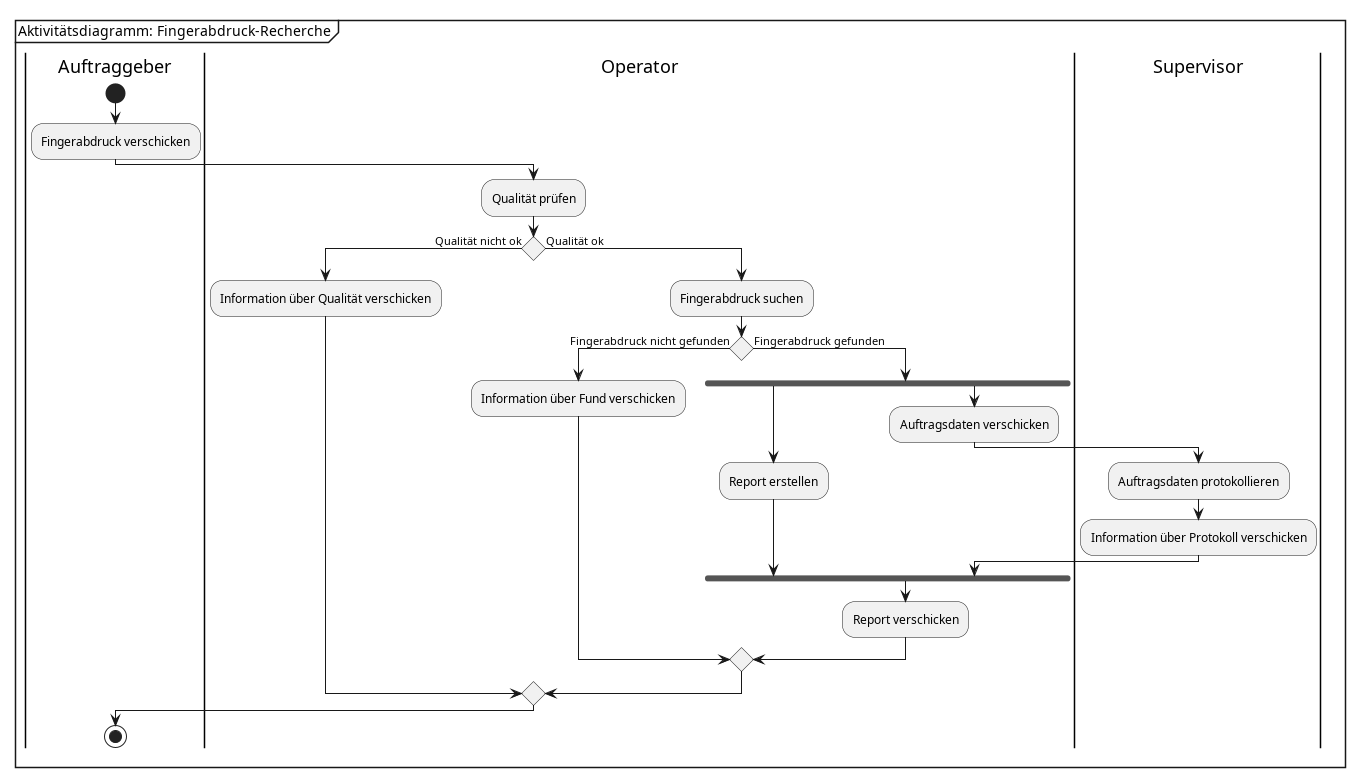
\includegraphics[width=\textwidth]{figures/activity.png}
    \caption{Beispiel Aktivitätsdiagramm}
\end{figure}

\subsection{Zustandsdiagramm}

\subsection{Sequenzdiagramm}

\subsection{Kommunikationsdiagramm}

\subsection{Zeitverlaufsdiagramm}

\subsection{Interaktionsübersichtsdiagramm}

\subsection{Profildiagramm}

\section{Struktogramm}

\chapter{Lernfeld 6: Serviceanfragen bearbeiten}

\textbf{Die Schülerinnen und Schüler verfügen über die Kompetenz, Serviceanfragen einzuordnen, Fehlerursachen zu ermitteln und zu beheben.}

Die Schülerinnen und Schüler nehmen Serviceanfragen entgegen (direkter und indirekter
Kundenkontakt). Sie \textbf{analysieren} Serviceanfragen und prüfen deren vertragliche Grundlage
(Service-Level-Agreement). Sie ermitteln die Reaktionszeit und dokumentieren den Status
der Anfragen im zugrundeliegenden Service-Management-System.

Durch systematisches Fragen \textbf{ordnen} die Schülerinnen und Schüler Serviceanfragen unter
Berücksichtigung des Support-Levels und fachlicher Standards \textbf{ein}.

Sie \textbf{ermitteln} Lösungsmöglichkeiten im Rahmen des Support-Levels. Auf dieser Basis \textbf{bearbeiten} sie das Problem und dokumentieren den Bearbeitungsstatus. Sie kommunizieren
mit den Prozessbeteiligten situationsgerecht, auch in einer Fremdsprache, und passen sich
den unterschiedlichen Kommunikationsanforderungen an (Kommunikationsmodelle, Deeskalationsstrategien).

Sie \textbf{reflektieren} den Bearbeitungsprozess der Serviceanfragen und ihr Verhalten in Gesprächssituationen. Die Schülerinnen und Schüler diskutieren die Servicefälle und schlagen
Maßnahmen zur Qualitätssteigerung vor.

\section{IT Service}

\subsection{ITSM - IT Service Management}

\subsection{ITIL - IT Infrastructure Library}

\subsection{Ticketsysteme}

\subsection{SLA - Service Level Agreements}

\subsection{Eisenhauer Matrix}

\subsection{Prozesskostenkalkulation}

\section{Projektplanung}

\subsection{Projektmanagement}

\subsection{4-Phasen Modell}

\subsection{Problemanalyse}

\subsection{Projektcanvas}

\subsection{Zielformulierung (SMART)}

\subsection{Risikoanalyse}

\subsection{Projektstrukturplan und Arbeitspakete}

\subsection{Gantt-Diagramm}

\subsection{Netzplantechnik}

Der Netzplan setzt eine Vorgangsliste (IDs, Vorgang, Dauer, Vorgänger) voraus. Vorgangsknoten werden im Netzplan durch Pfeile in Abhängigkeit dargestellt. Der kritische Pfad ergibt sich aus der geringsten Projektzeit, erkennbar an den Vorgängen ohne Puffer.

\begin{figure}
    [H]
    \centering
    \begin{tabular}{|c|c|c|}
        \multicolumn{1}{c}{FAZ} & \multicolumn{1}{c}{}         & \multicolumn{1}{c}{FEZ} \\\hline
        ID                      & \multicolumn{2}{c|}{Vorgang}                           \\\hline
        D                       & GP                           & FP                      \\\hline
        \multicolumn{1}{c}{SAZ} & \multicolumn{1}{c}{}         & \multicolumn{1}{c}{SEZ} \\
    \end{tabular}
    \caption{Vorgangsknoten}
\end{figure}

\begin{itemize}
    \item D = Dauer
    \item FAZ = Frühester Anfangszeitpunkt (Bei erstem Vorgang null, sonst größter FEZ der Vorgänger)
    \item FEZ = Frühester Endzeitpunkt (FAZ + D)
    \item SAZ = Spätester Anfangszeitpunkt (SEZ - D)
    \item SEZ = Spätester Endzeitpunkt (Bei letztem Vorgang null, sonst kleinster SAZ der Nachfolger)
    \item GP = Gesamtpuffer (Summe der Puffer der Nachfolger; SAZ - FAZ)
    \item FP = Freier Puffer (Puffer des Vorgangs; kleinster FAZ der Nachfolger - FEZ)
\end{itemize}

\begin{table}
    [H]
    \centering
    \begin{tabular}{|c|l|c|c|}
        \hline
        \textbf{ID} & \textbf{Vorgang}                & \textbf{Dauer} & \textbf{Vorgänger} \\\hline
        1           & Infrastruktur ermitteln         & 1              & -                  \\\hline
        2           & Arbeitsplatzbedarf ermitteln    & 2              & 1                  \\\hline
        3           & Netzwerkplan entwerfen          & 1              & 1                  \\\hline
        4           & Peripheriebedarf ermitteln      & 1              & 3                  \\\hline
        5           & Hardware PC + Server beschaffen & 4              & 2                  \\\hline
        6           & Software beschaffen             & 2              & 5                  \\\hline
        7           & Netzwerkzubehör beschaffen      & 2              & 3; 5               \\\hline
        8           & Peripherie beschaffen           & 1              & 4                  \\\hline
        9           & Hardware PC + Server aufbauen   & 6              & 5                  \\\hline
        10          & Server installieren             & 3              & 9                  \\\hline
        11          & Netzwerk aufbauen               & 5              & 7                  \\\hline
        12          & PC-Image anlegen                & 1              & 6; 10; 11          \\\hline
        13          & Peripherie anschließen          & 1              & 8; 10; 11          \\\hline
        14          & Netzwerkplan dokumentieren      & 2              & 13                 \\\hline
        15          & Server-Image anlegen            & 1              & 10                 \\\hline
        16          & PC-Remote installieren          & 1              & 12                 \\\hline 17 & Gesamtdokumentation erstellen & 3 & 14; 15; 16 \\\hline
    \end{tabular}
    \caption{Beispiel Vorgangsliste}
\end{table}

\begin{figure}[H]
    \centering
    \includesvg[width=\textwidth,inkscapelatex=false]{figures/Netzplan.drawio.svg}
    \caption{Beispiel Netzplan anhand der Vorgangsliste}
\end{figure}
\FloatBarrier

\chapter{Lernfeld 9: Netzwerke und Dienste bereitstellen}

\textbf{Die Schülerinnen und Schüler verfügen über die Kompetenz, Netzwerke und Dienste
    zu planen, zu konfigurieren und zu erweitern.}

Die Schülerinnen und Schüler ermitteln die Anforderungen an ein Netzwerk in Kommunikation mit den Kunden. Sie \textbf{informieren} sich über Eigenschaften, Funktionen und Leistungsmerkmale der Netzwerkkomponenten und Dienste nach Kundenanforderung, auch unter
Berücksichtigung sicherheitsrelevanter Merkmale. Dabei wenden sie Recherchemethoden
an und werten auch fremdsprachliche Quellen aus.

Sie \textbf{planen} die erforderlichen Dienste und dafür notwendige Netzwerke sowie deren Infrastruktur unter Berücksichtigung interner und externer Ressourcen.

Dazu \textbf{vergleichen} sie Konzepte hinsichtlich ihrer Nachhaltigkeit sowie der technischen und
wirtschaftlichen Eignung.

Sie \textbf{installieren} und konfigurieren Netzwerke sowie deren Infrastruktur und implementieren
Dienste. Sie gewährleisten die Einhaltung von Standards, führen Funktionsprüfungen sowie
Messungen durch und erstellen eine Dokumentation.

Die Schülerinnen und Schüler \textbf{beurteilen} die Netzwerke sowie deren Infrastruktur und die
Dienste hinsichtlich der gestellten Anforderungen, Datensicherheit und Datenschutz.

Sie \textbf{reflektieren} ihre Lösung unter Berücksichtigung der Kundenzufriedenheit, Zukunftsfähigkeit und Vorgehensweise.

Die folgenden Informationen beschäftigen sich hauptsächlich mit Netzwerksoftware. Für Netzwerkhardware, Struktur und Physik siehe Lernfeld 3.

\section{Netzwerksoftwaremodelle}

Netzwerke sind meist in hierarchische Schichten (Layers) aufgeteilt. Jede Schicht bietet den höheren Schichten bestimmte Services und kümmert sich alleine um die Implementation dieser Services.

Die Kommunikation findet dabei in der Theorie in den einzigen Schichten statt und wird von Protokollen dieser Schichten geregelt.

\begin{figure}[H]
    \centering
    \includesvg[width=\textwidth,inkscapelatex=false]{figures/Netzwerkmodell.drawio.svg}
    \caption{Beispiel Schichtmodell allgemein}
    \label{fig:schichtmodell}
\end{figure}
\FloatBarrier

Ein Host hat pro Schicht eine Kommunikationskomponente gen. Peer, die mit einem Peer der gleichen Schicht eines anderen Hosts kommunizieren kann. Praktisch sind Peers z.B. Softwareprozesse, Hardwaregeräte oder Menschen.

Praktisch findet die Kommunikation nicht horizontal innerhalb der einzelnen Schichten, sonder vertikal zwischen den Schichten statt. Jede Schicht fügt Informationen hinzu, die für ihr Protokoll notwendig sind. Die Übertragung findet auf der untersten Schicht in einem physischen Medium statt.

Zwischen zwei Schichten definieren Schnittstellen (Interfaces) ähnlich Blaupausen welche Services die untere Schicht anbieten sollte.

Eine Menge an Schichten und Protokollen wird als Netzwerkarchitektur bezeichnet. Eine Liste an Protokollen mit einem Protokoll für jede Schicht wird als Protokollstack bezeichnet.

Protokolle benötigen mindestens Steuerinformationen zusätzlich zu den eigentlichen Nutzdaten. Jedes Protokoll fügt Informationen hinzu und gibt seine Nutzdaten plus die zusätzliche Informationen an das untere Protokoll als seine Nutzdaten weiter. Dieser Vorgang läuft auf der Zielmaschine Rückwärts ab. Das zugrunde liegende Prinzip nennt sich Datenkapselung.

\begin{figure}[H]
    \centering
    \includesvg[width=\textwidth,inkscapelatex=false]{figures/Datenkapselung.drawio.svg}
    \caption{Beispiel Datenkapselung im Netzwerkmodell}
    \label{fig:Datenkapselung}
\end{figure}
\FloatBarrier

\subsection{ISO Open Systems Interconnection Referenzmodell (OSI-Modell)}

Das OSI-Modell ist keine Netzwerkarchitektur aber eine Vorlage für diese. Die einzelnen Schichten sind nach Funktionen getrennt.

\begin{table}[H]
    \centering
    \begin{tabular}{|l|l|}
        \hline
        7 & Application/ Anwendung    \\\hline
        6 & Presentation/ Darstellung \\\hline
        5 & Session/ Sitzung          \\\hline
        4 & Transport                 \\\hline
        3 & Network/ Vermittlung      \\\hline
        2 & Data Link/ Sicherung      \\\hline
        1 & Physical/ Bitübertragung  \\\hline
    \end{tabular}
    \caption{ISO OSI-Modell Übersicht}
\end{table}

\begin{figure}[H]
    \centering
    \includesvg[width=\textwidth,inkscapelatex=false]{figures/OSI_allgemein.drawio.svg}
    \caption{OSI-Modell}
\end{figure}
\FloatBarrier

\begin{table}
    [H]
    \centering
    \begin{tabularx}{\textwidth}{|c|l|l|>{\raggedright\arraybackslash}X|>{\raggedright\arraybackslash}X|>{\raggedright\arraybackslash}X|>{\raggedright\arraybackslash}X|}
        \hline
        \textbf{ID} & \textbf{OSI}                     & \textbf{TCP/IP} & \textbf{Protokolle u. Techniken}  & \textbf{Einheiten} & \textbf{Kopplung}            & \textbf{Verbindung} \\\hline
        7           & Application                      & Application     & DHCP, DNS, FTP, HTTP, HTTPS, SMTP & Daten              & Gateway, Proxy               & Ende zu Ende        \\\cline{1-2}
        6           & Presentation                     &                 &                                   &                    &                              &                     \\\cline{1-2}
        5           & Session                          &                 &                                   &                    &                              &                     \\\cline{1-5}
        4           & \multicolumn{2}{c|}{Transport  } & TCP, UDP        & Segmente, Datagramme              &                    &                                                    \\\cline{1-6}
        3           & Network                          & Internet        & ICMP, IP                          & Pakete             & Router                       &                     \\\cline{1-7}
        2           & Data Link                        & Link            & Ethernet, WLAN, MAC               & Frames             & Bridge, Switch, WAP          & Punkt zu Punkt      \\\cline{1-2}\cline{5-6}
        1           & Physical                         &                 &                                   & Bits, Symbole      & Netzwerkkabel, Repeater, Hub &                     \\\hline
    \end{tabularx}
    \caption{Vollständige Übersicht OSI und TCP/IP}
\end{table}

\subsection{Transmission Control Protocol/ Internet Protocol (TCP/IP)}

Der TCP/IP-Stack ist die Gruppierung von Netzwerkprotokollen. Im weiteren Sinne der gesamte Stack für die Internetprotokollfamilie.

Der Stack wird u.a. im TCP/IP-Referenzmodell dargestellt. Das Modell gilt damit als darstellung der TCP/IP-Netzwerkarchitektur.

\begin{table}
    [H]
    \centering
    \begin{tabular}{|l|l|l|}
        \hline
        \multicolumn{2}{|l|}{\textbf{Schicht}} & \textbf{Besipielprotokolle}                                      \\\hline
        4                                      & Application/ Anwendung      & HTTP, UDP, FTP, SMTP, Telnet, DHCP \\\hline
        3                                      & Transport                   & TCP, UDP                           \\\hline
        2                                      & Internet                    & IP, ICMP                           \\\hline
        1                                      & Link/ Netzzugang            & \multicolumn{1}{c}{}               \\\cline{1-2}
    \end{tabular}
    \caption{TCP/IP-Modell Übersicht}
\end{table}

Die \textbf{Anwendungsschicht} befasst sich hier mit Protokollen für Anwendungsprogramme und die Netzinfrakstruktur für anwendungsspezifischen Datenaustausch.

Die \textbf{Transportschicht} befasst sich mit der Ende-zu-Ende-Kommunikation.

Die \textbf{Internetschicht} befasst sich mit der Übertragung von Paketen und der Wegwahl (Routing) dieser. Auf dieser Schicht und der Netzzugangsschicht werden Direktverbindungen betrachtet.

Die \textbf{Netzzugangsschicht} beinhaltet keine Protokolle per se sondern ist ein Platzhalter für Techniken der Datenübertragung von Punkt zu Punkt.

\section{IPv4}

\end{document}